\documentclass[10pt,a4paper]{article}

\usepackage[utf8]{inputenc}
\usepackage{graphicx}
\usepackage{gensymb}
\usepackage{amsmath}
\usepackage{amssymb}
\usepackage{geometry}
\usepackage{multicol}  
\usepackage{siunitx}
\usepackage{float}
\usepackage{color}
\graphicspath{{../figures/}}

\geometry{a4paper}

\author{Nik Dennler \\ Johannes Lade}
\title{Digital Electronics Lab\\ \textbf{Exercises}}
\date{\today{}}


\begin{document}
	
\begin{titlepage}
	\maketitle
		\begin{center}
			Email: nik.dennler@uzh.ch, johannes.lade@uzh.ch
		\end{center}
	\thispagestyle{empty}
\end{titlepage}




\section{Exercise Block 1}
\label{sec:exercise-block-1}

\subsection{Exclusive OR (30min)}\label{subsec:ex-1}

XOR stands for exclusive OR. As the name suggest, it is very similar to the OR gate, except that it does not yield one when both inputs are one. In different words this means that the XOR is true whenever the two inputs are not equal. Follow the steps below to construct the XOR circuit.
\begin{enumerate}
	\item Write down the truth table.
	\item\label{it:1} Construct the disjunctive normal form from your truth table.
	\item Draw the circuit from the disjunctive normal form.
	\item Transform the circuit in such a way that it only uses NAND Gates.
	\item How many NAND gates do you need? See if you can loose one or two gates.
\end{enumerate}

\subsection{XOR to the Next (30min)}
Only start this exercise once you showed your circuit diagram to one of the assistants.
Construct the XOR gate on the breadboard.

\section{Excercise Block 2}

\subsection{Half-Adder (30min)}
\subsubsection{Part 1}
A half-adder takes two bits $a$ and $b$ and adds them. It is called half-adder because two of them are needed in order to construct an adder which is able to add several bits. We will see later why this is the case.

Let's first look at the addition of two decimal digits. 

\begin{figure}[h]
	\centering		  
	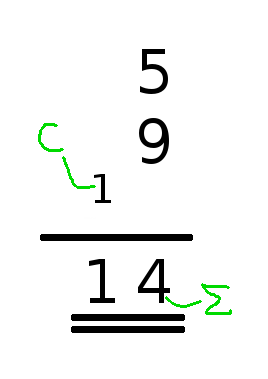
\includegraphics[scale=0.3]{decimal_addition.png}
	\caption{Decimal addition.}
	\label{fig:decimal_addition}
\end{figure}
We see that we need two things:
\begin{itemize}
	\item In the rightmost column we need to know in which digit the addition of 5 and 9 results. $5+9=14$. But in the same column we only write the part of the number which does not exceed $10$. Namely $4$. We call this the sum and denote it with $\Sigma$.
	\item In the next column we need to carry a 1 because $5+9$ exceeds 10. We call this the carry digit and denote it with $C$.
\end{itemize}

For binary digits (bits) we can do the same thing. Let's assume the following case. We have two 1 digit binary numbers. We call the single bit of the first number $a$ and the single bit of the second number $b$.
\begin{itemize}
	\item Write down all possible combinations of $a$ and $b$ in table \ref{tab:half-adder-truth-table}.
	\item Think about the output of each combination of $a$ and $b$ and write it into table \ref{tab:half-adder-truth-table} in the column $\Sigma$ (for sum). Remember that a bit can never exceed one but instead wraps back to zero just as 9 does when you add 1 in the decimal system. 
	\item Similar to the decimal case, we need to sometimes carry a bit. Write the value of the carry bit $C$ into table \ref{tab:half-adder-truth-table}.
	\item Now look at the columns of $\Sigma$ and $C$. Which logical circuits do they represent?
	
	\begin{table}[H]
		\centering
		\begin{tabular}{|c|c||c|c|}
			\hline
			$a$ & $b$ & $\Sigma$   & $C$ \\ \hline
			&     &           &       \\ \hline
			&     &           &       \\ \hline
			&     &           &       \\ \hline
			&     &           &       \\ \hline
		\end{tabular}
		\caption{Truth table for the Half Adder.}
		\label{tab:half-adder-truth-table}
	\end{table}
	
		\item Draw the two circuits from table \ref{tab:half-adder-truth-table} and reduce them to NAND representation without actually building them. (Hint: One of the two circuits you know already. Use the reduced form from the last exercise.)
		\item With the two circuits drawn entirely with NAND gates, see if you can combine them into one.
		\item Congrats, you have successfully drawn the circuit of a half adder. Ask an assistant wether it is correct. Now build one on the breadboard.
\end{itemize}
\subsection{Full-Adder (30min)}
You may have noticed that the half-adder - although you can add two bits and generate a carry bit - is not enough to add several bits together.

Because, how much use is a carry bit generatated by one circuit if we cannot use it in the next one? This means we need to be able to operate on three inputs: $a$, $b$ and $C_{in}$ (See figure \ref{fig:full-binary-addition}). The half-adder cannot do that\footnote{For a more elaborate explanation see section \ref{subsec:appendix-full-adder} in the appendix.}.

\begin{figure}[H]
	\centering		  
	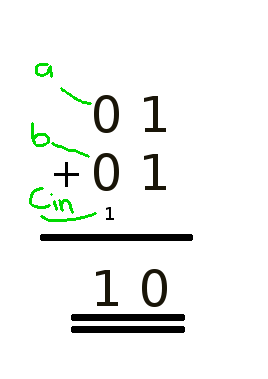
\includegraphics[scale=0.3]{full_binary_addition.png}
	\caption{Full binary addition.}
	\label{fig:full-binary-addition}
\end{figure}






Lukily the full-adder - which can add three single bits - is easily built with two half-adders, hence the name. As the derivation of the full adder is beyond the scope of this lecture, we will simply introduce its logic circuit. For simplicity we pack the circuit of the half adder into one black box and simply denote its outputs with $\Sigma$ and $C$ (See figure \ref{fig:full-adder}).

So now we are able to add three single bits: $a$, from the first number, $b$, from the second number and $C_{in}$, the carry bit from the last summation. 

\begin{figure}[H]
	\centering		  
	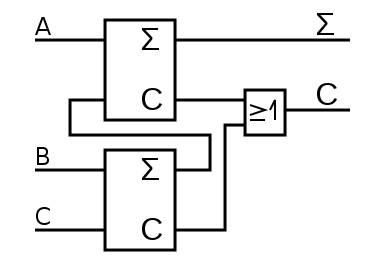
\includegraphics[scale=0.3]{full_adder.png}
	\caption{Full adder built of two half-adders.}
	\label{fig:full-adder}
\end{figure}
\begin{itemize}
	\item Fill in all possible combinations for $C_{in}$, $a$ and $b$ in table \ref{tab:full-adder-truth-table}. Think about what $\Sigma$ and $C_{out}$ should be and fill them in as well.
	\item Visually test the circuit drawing for all possible combinations and compare it with your expectations for $\Sigma$ and $C_{out}$. Do they match?
	
	\begin{table}[h]
		\centering
		\begin{tabular}{|c|c|c||c|c|}
			\hline
			$C_{in}$ & $a$ & $b$ & $\Sigma$ & $C_{out}$ \\ \hline
			&     &     &          &           \\ \hline
			&     &     &          &           \\ \hline
			&     &     &          &           \\ \hline
			&     &     &          &           \\ \hline
			&     &     &          &           \\ \hline
			&     &     &          &           \\ \hline
			&     &     &          &           \\ \hline
			&     &     &          &           \\ \hline
		\end{tabular}
		\caption{Truth table for the Full Adder.}
		\label{tab:full-adder-truth-table}
	\end{table}
	
	\item Once you have convinced yourself that the circuit is correct, translate it into only NAND gates by using the half-adders you derived earlier. (Hint: Do not transform the OR gate until the very end. You will see that it simplifies very easily into a NAND gate.)
	\item Build the full adder on the breadboard.
\end{itemize}

\subsection{Combine Full Adders}
If you successfully built your full adder, show it to an assistant. Now you are ready to join up with three other groups in order to combine your full adders to a fully functional 4 bit adder (See figure \ref{fig:4bit}). The assistant will show you how.
\begin{figure}[H]
	\centering		  
	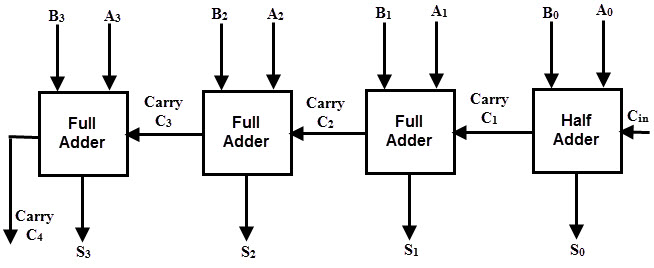
\includegraphics[scale=0.5]{4bit}
	\caption{Logic circuit of a 4 bit adder.}
	\label{fig:4bit}
\end{figure}


\section{Additional Exercise (Only if you got time)}
In figure \ref{fig:RSFF} you see a logic circuit that is called an RS Flip-Flop. Try to find out what it does, either with a truth table or by building it. If you need help, ask an assistant.

\begin{figure}[H]
	\centering
	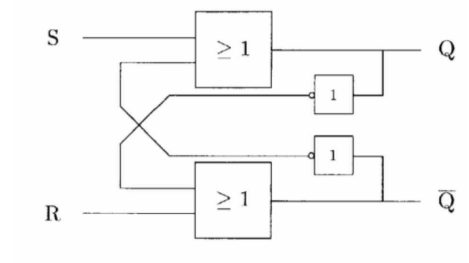
\includegraphics[height=0.35\textwidth]{RSFF}%
	\caption{RS-Flip-Flop}%
	\label{fig:RSFF}
\end{figure}

\section{Appendix}
\subsection{Full Adder}\label{subsec:appendix-full-adder}

Look at two 2 bit numbers: For example $01_2$ and $11_2$\footnote{The subscript denotes the number system in wich we write the number. So that we may know that $11_2$ means three and not eleven.}.  We call them $01_2 = a_1a_0$ and $11_2 = b_1b_0$. Then the half-adder is enough in order to add the first two bits $a_0$ and $b_0$. The results is $\Sigma=0$ and $C=1$. But as soon as we want to add the next two bits $a_1$ and $b_1$ we also need to add the carry bit $C$ from the first operation. So we have $a_1+b_1+C = 0 + 1 + 1$, but the half-adder is not capable of adding three bits. Consequently, if we were to build a two bit adder only with half-adders then the carry bits would just be ignored. This would lead to wrong results like this:
\[
a_1a_0 + b_1b_0 = 01_2 + 11_2 = 10_2
\]
or in decimal
\[
1_{10} + 3_{10} = 2_{10}
\]
\end{document}



